We target CLEF-IP 2010 and 2011 collections\footnote{\url{http://www.ifs.tuwien.ac.at/~clef-ip/}}
for our research. CLEF-IP 2010 is a set of patents from the `European Patent Office' (EPO), and CLEF-IP 2011 includes the same patent data collection from EPO, but with the addition of a new set of patents from `World Intellectual Property Organization' (WIPO). CLEF-IP 2010 contains 2.6 million patent documents and CLEF-IP 2011 consists of 3 million patent documents. The English test sets of CLEF-IP 2010 and CLEF-IP 2011 correspond to 1303 and 1351 topics respectively.

Each patent in the collection consists of multiple versions of documents in the XML format, labelled as A1, A2, $\ldots$, B1, and B2. The letter 'A' refers to different versions of patent applications. The 'B' versions refer to granted patents. Each of these versions contains some updates to the text, citations, and claims of previous one. As recommended by~\cite{magdy2012toward}, we merge different versions of a single patent into one single document. The content of each section in the merged document is taken from the latest available versions of documents, which leads to presence of some patents in the collection with many missing content fields. The problem of missing data is in some cases so significant that some of these patents consist only of title.

The patent collections contain material in three different languages: English, German, and French. Granted published version of a patent (i.e., the 'B' version) by the EPO should contain the claims section manually translated into all three languages. In addition, all patents have the title in the three languages. The description section of all patents is always provided in the original submission language only.

Test topics provided are English, German, and French patent applications, which are used as a query for the retrieval system. Topics for CLEF-IP 2010 are patent applications rather than granted patents as in 2009. Therefore, non-English patent applications did not contain any English translations in any section except the title and the abstract. However, in CLEF-IP 2010, 1302 out of 1303 test topics were English and only one was German. 

Figure~\ref{fig:lang-a} shows the percentage of the English, German, and French patents in the CLEF-IP 2010 collection. Since some patents in the collection do not contain all sections, and since some of the non-English patents do not contain translations into English, Figure~\ref{fig:lang-b} presents the distribution of the missing English sections in the patents. Figure~\ref{fig:lang-b} shows the amount of the English content present in the patents in the 2010 collection, where only 52\% of the patents in the collection were complete English documents. 16\% of the collection included the titles and claims sections only, while some of them contained the abstract section as well. These patents are not complete patent documents, but at the same time, they are not short because of the presence of the claims section which contains most of the important information about the invention disclosed. 32\% of the patents do not include the description or the claims sections in English, while most of them included the titles only, which means that the retrievability of these patents is expected to be very low, since they contain only a very small number of words. The overall aim of Figure~\ref{fig:lang-b} is to show that the documents in the patent collection are not homogeneous since many of them are in some respect incomplete~\citep{magdy2012toward}.
%%%%%%%%%%%%%%%%%%%%%%%%%%%%%%%%%%%%%%%%%%%%%%%%%%%%%%%%%%%%%%
\begin{figure}[t!]
\begin{centering}
%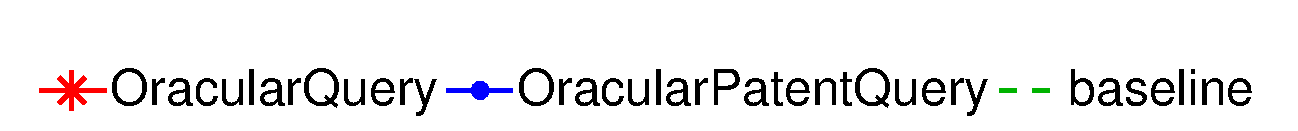
\includegraphics[width=9cm]{imgs/l1}
\par\end{centering}

\begin{centering}
\subfigure[{}\label{fig:lang-a}]{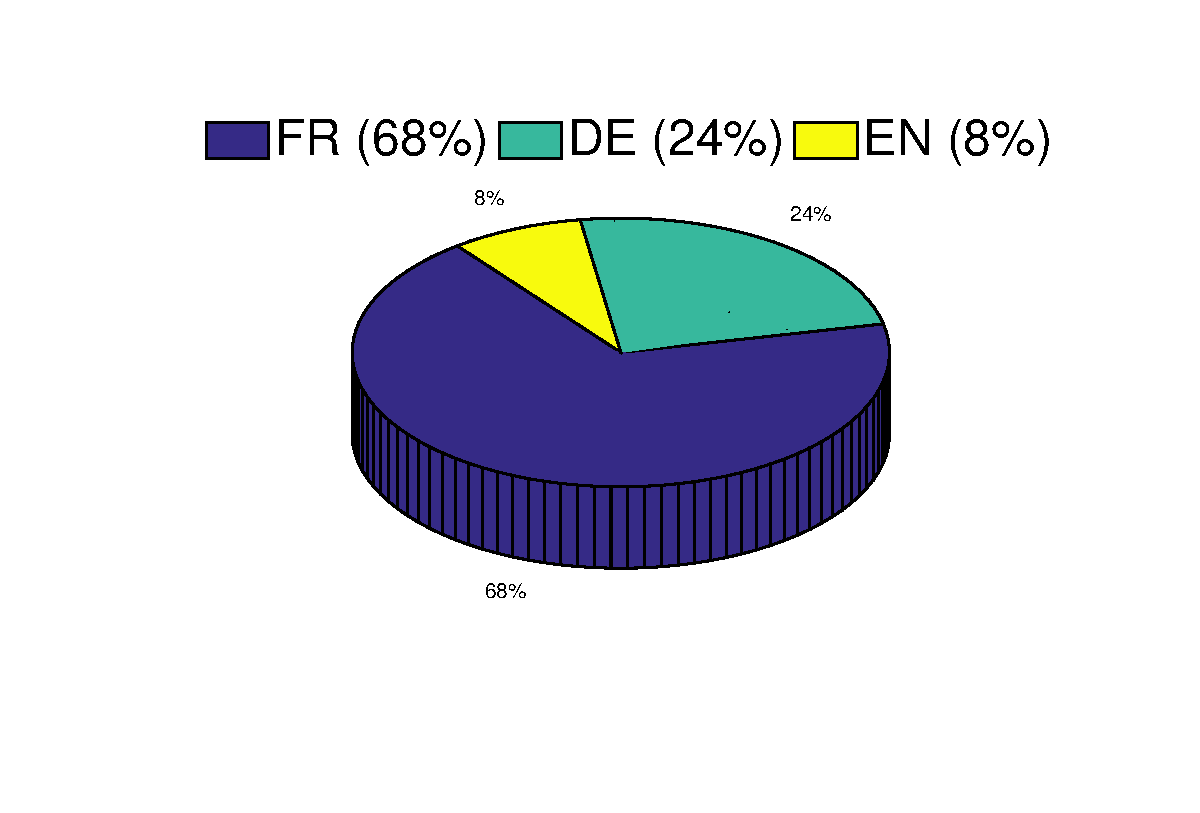
\includegraphics[width=8cm]{figs/lang1.eps}}\subfigure[\label{fig:lang-b}]{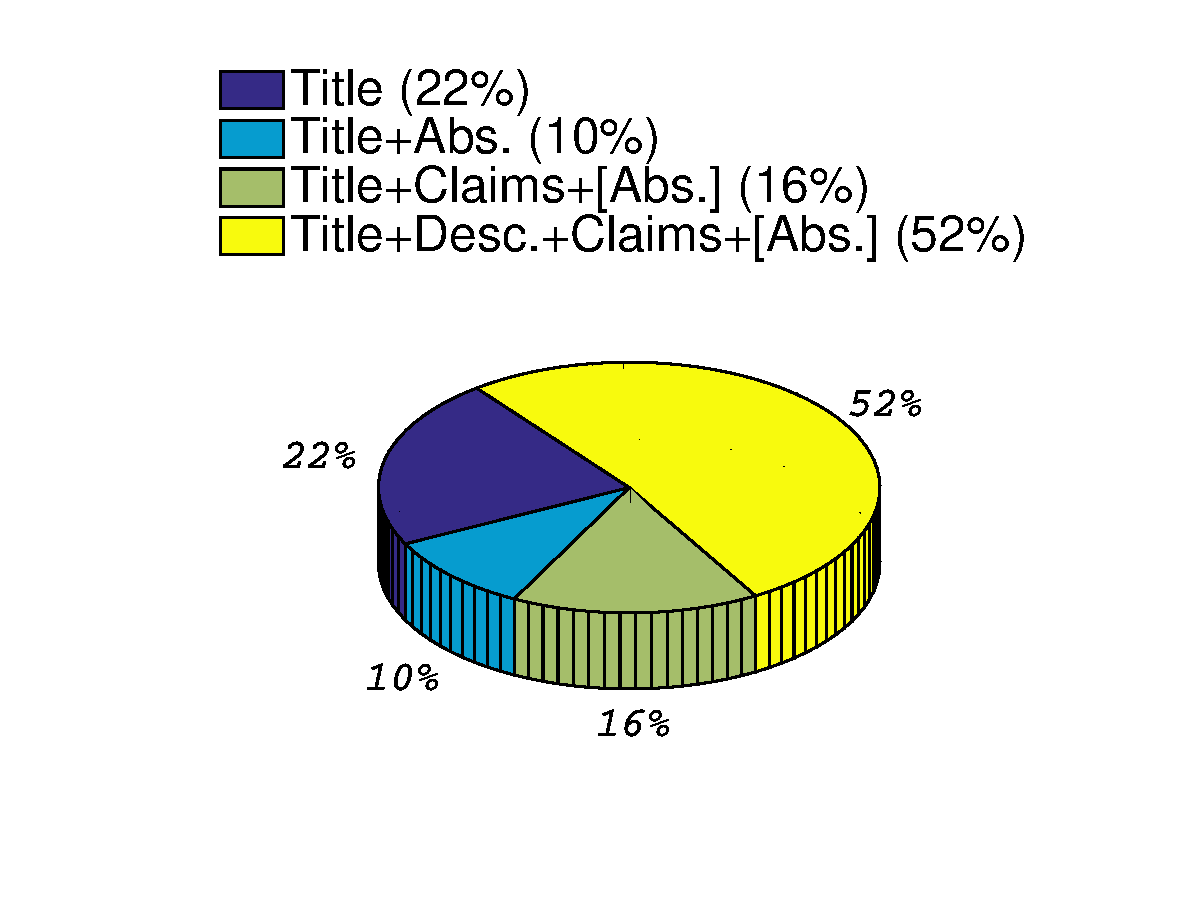
\includegraphics[width=8cm]{figs/lang2.eps}}
\par\end{centering}
\vspace{1mm}
\protect\caption{(a) Percentage of English, German, and French patents in CLEF-IP 2010 collection.
                 (b) Completeness of the presence of English text in the CLEF-IP 2010 patent collection.~\citep{magdy2012toward}.}
\label{fig:lang}
\end{figure}
%%%%%%%%%%%%%%%%%%%%%%%%%%%%%%%%%%%%%%%%%%%%%%%%%%%%%%%%%%%%%%
%\begin{figure}[t!]
%\begin{centering}
%\subfigure[\label{fig:lang-a}]{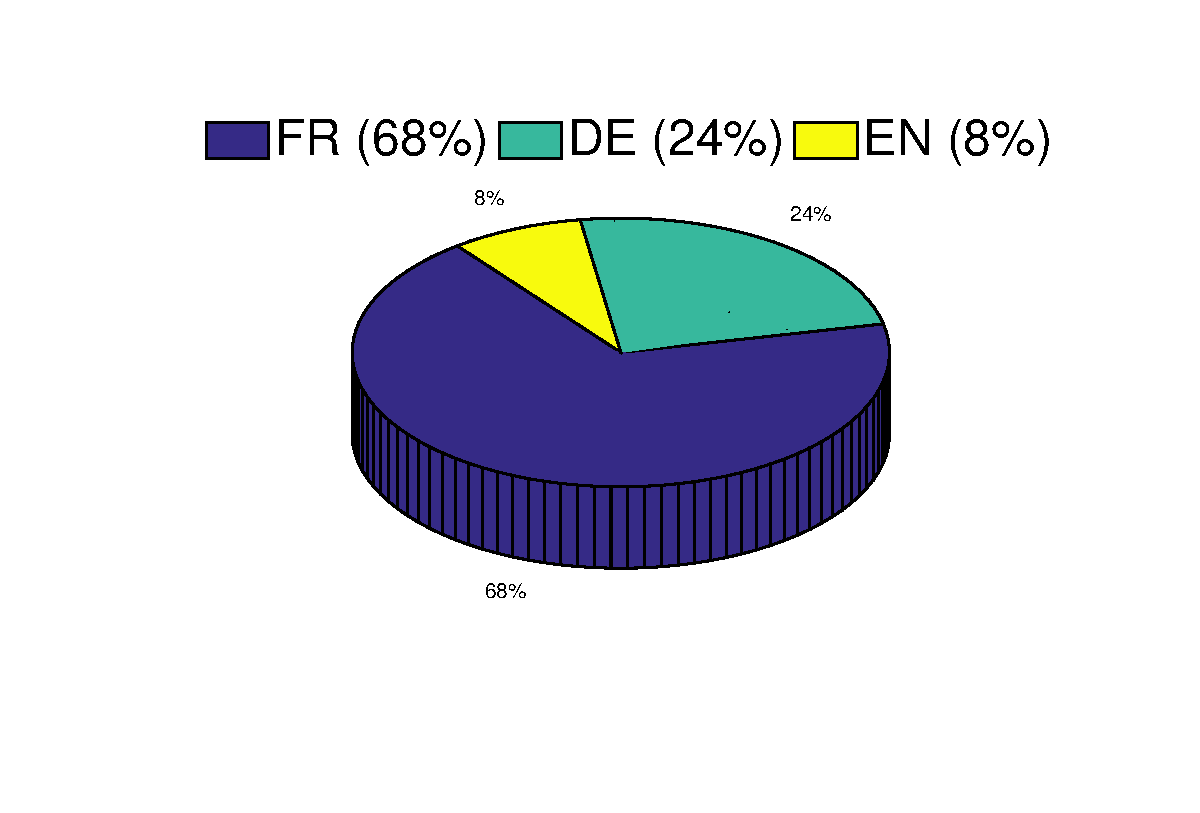
\includegraphics[width=4cm]{figs/lang1.eps}} \hspace*{1.5cm} 
%\subfigure[\label{fig:lang-b}]{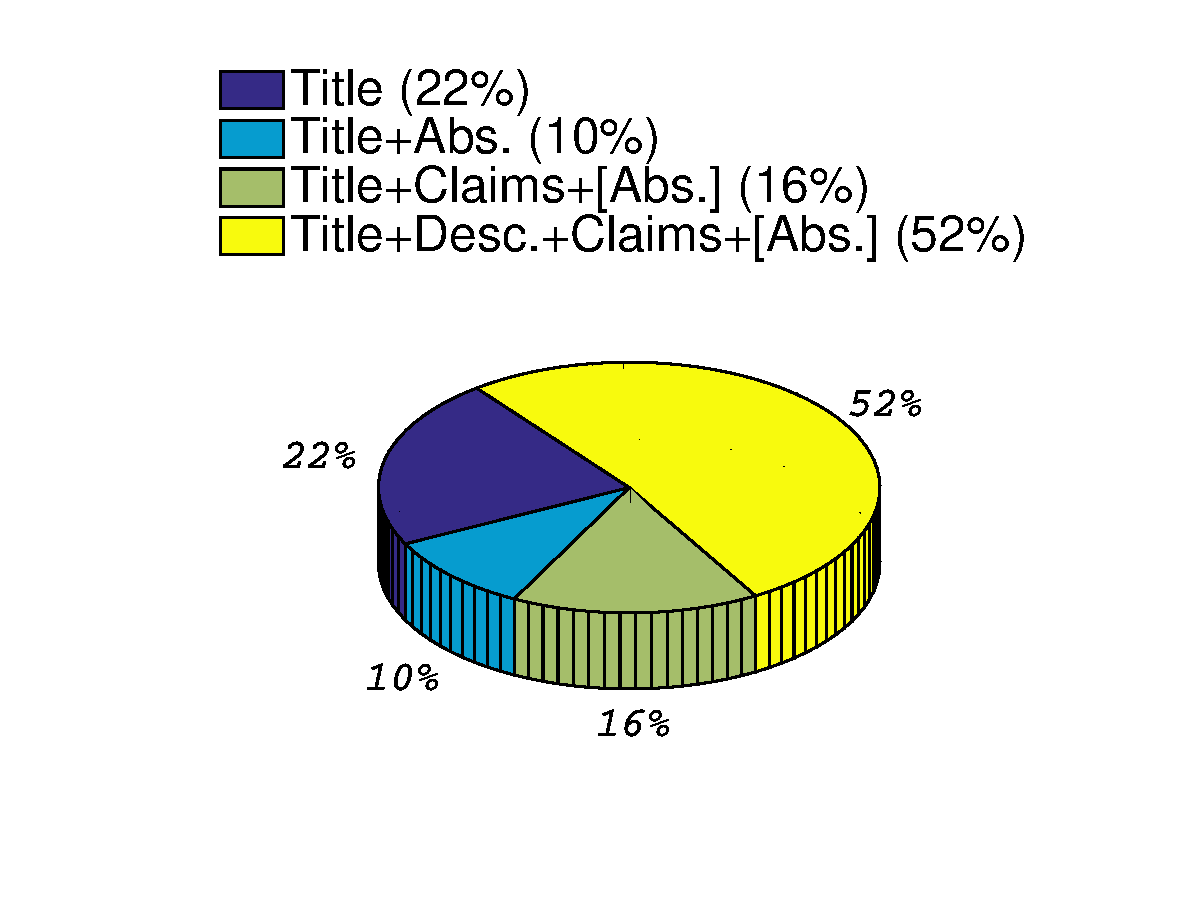
\includegraphics[width=6.5cm]{figs/lang2.eps}} 
%\par\end{centering} 
%\protect\caption{(a) Percentage of English, German, and French patents in CLEF-IP 2010 collection.
%                (b) Completeness of the presence of English text in the CLEF-IP 2010 patent collection.~\citep{magdy2012toward}}
%\label{fig:lang}
%\end{figure}
